
%%%%%%%%%%%%%%%%%%%%%%%%%%%%%%%%%%%%%%%%%%%%%%%%%%%%%%%%%%%%%%%%%%%%%%

\section{Analysis}
\label{sec:analysis}
\label{sec:theorems}

We analyze the impact of task creation overheads on parallel execution
time and show how these costs can be reduced dramatically by using our
oracle semantics.  For our analysis, we first consider an {\em ideal
  oracle} that always makes perfectly accurate predictions (about the
raw work of expressions) without any overhead (\textit{i.e.}, $\corc = 0$).
Such an ideal oracle is unrealistic, because it is practically
impossible to determine perfectly accurately the raw work of
computations.  We therefore consider a realistic oracle that
approximates the raw work of computations by performing constant work.
Our main result is a theorem that shows that the ideal oracle can
reduce the task-creation overheads to any desired constant fraction of
the raw work with some increase in depth, which we show to be small
for a reasonably broad class of computations.

\subsection{Ideal oracle}

We quantify the relationships between raw work, raw depth and
total work, total depth for each mode.

\begin{theorem}[Work and depth]
\label{thm:work-depth-all}
Consider an expression $e$ such that $\Jcostof{\Ga}{ e }{v}{\sw}{\sd}{\sws}{\sds}$.
Assume $\corc = 0$.
The following tight bounds can be obtained for total work and total depth,
on a machine with $P$ processors where the cost of creating parallel tasks is $\csp$.
%
$$\begin{array}{c|c|c} %|l
\X{$\Ga$} & 
\X{Bound on total work} &
\X{Bound on total depth} 

\\\hline
\sseq & 
\sws = \sw &
\sds = \sd = \sw 

\\\hline
\spar & 
\sws \leq (1+\frac{\csp}{2})\,\sw &
\sds \leq (1+\csp)\,\sd 

\\\hline
\sorc & 
\sws \leq (1 + \frac{\csp}{\coff+1})\,\sw &
\sds \leq (1+\kwmax{\csp}{\coff})\,\sd 
\end{array}$$

\end{theorem}

\begin{proof}
The equations concerning the sequential semantics follow by inspection
of the semantics of the source language (\figref{src-sem}).  The
inequalities for the parallel and the oracle modes follow directly by
our more general bounds presented later
(\thmreftwo{orc-cost-depth}{orc-cost-work}).  To prove that the
inequalities for the parallel and the oracles modes are tight, we give
example computation that achieve the bounds.

\begin{itemize}
\item \textbf{Parallel mode.}  Consider an expression consisting only
  of parallel tuples with $n$ leaves, and thus $n-1$ ``internal
  nodes''.  The raw work $\sw$ is equal to $n+(n-1)$ while the total
  work $\sws$ is equal to $n+(n-1)(1+\csp)$.  We therefore have $\sws
  = (1+\frac{n\csp}{2n+1})\sw \le \left(1+\frac{\tau}{2}\right)
  \sw$. As $n$ increases, the bound approaches
  $\left(1+\frac{\tau}{2}\right) \sw$ and thus the bound on the total
  work is tight. To see that the depth bound is also tight, note that
  each parallel tuple adds~$1$ to the raw depth and~$1+\csp$ to the
  total depth.  The total depth therefore can be as much as $1+\csp$
  times greater than the raw depth.

\item \textbf{Oracle mode.}  
Consider an expression with~$n$ nested parallel tuples, where tuples
are always nested in the right branch of their parent tuple.  The
tuples are built on top of expressions that involve~$\coff$ 
units of work.  In the oracle semantics, all the tuples
are executed in parallel.  Thus the raw work~$\sw$ is $n +
(n+1)\coff$, the total work~$\sws$ is $n (1+\csp) +
(n+1)\coff$, and $\sws = \sw \left( 1 + \frac{n\csp}{n(\coff+1)+\coff}
\right) \le \sw \left( 1+\frac{\csp}{\coff+1} \right)$.  As~$n$
increases, the bound approaches $\left(1+\frac{\csp}{\coff + 1}\right) \sw$
and thus the bound on the total work is tight.  

For the depth bound, we  consider two cases.  In the first case,
we have~$\csp \geq \coff$.  Using the same example, the raw depth is~$
\sd = n+1$, the total depth is~$\sds = n(1+\csp) + \coff$, and $\sds =
\left( 1+\frac{n\csp+\coff-1}{n+1} \right) \sd \le \left( 1+\csp
\right) \sd$.  As~$n$ increases,~$\sds$ approaches~$\left( 1+\csp
\right) \sd$ and thus the bound is tight.

For the second case when $\coff\geq\csp$, we change the example
slightly by reducing the amount of raw work in each leaf to just
under $\coff$.  This will cause all the parallel tuples to be
evaluated sequentially; the raw depth is $\sd = n+\coff$ and the
total depth is equal to the total work, \textit{i.e.}, $\sds = n+(n+1)\coff \le
\left( 1+\frac{n\coff}{n+\coff} \right) \sd$.  As $n$ increases, $\sds$
approaches $\left( 1+\coff \right) \sd$ and thus the
bound is tight. \qed
\end{itemize}
\end{proof}

This theorem leads to some important conclusions.  First, the theorem
shows that task creation (scheduling) costs matter a great deal.  In a
parallel evaluation, the total work and total depth can be as much as
$\csp$~times larger than the raw depth and raw work.  This essentially
implies that a parallel program can be significantly slower than its
sequential counterpart.  If $\csp$ is large compared to the number of
processors, then even in the ideal setting, where the number of
parallel processors is small relative to $\csp$, we may observe no
speedups.  In fact, it is not uncommon to hear anecdotal evidence of
this kind of slowdown in modern computer systems.

%\mremark{It'd help to recall the definition of parallel slackness
%  before we use it below, as we have not yet defined the term
%  precisely.}

Second, the theorem shows that evaluation of a program with an ideal
oracle can require as much as $\frac{\coff}{2}$ less work than in the
parallel mode.  This comes at a cost of increasing the depth by a
factor of $\frac{\coff}{\csp}$.  Increasing the depth of a computation can
hurt parallel execution times because many parallel schedulers rely on
the availability of large degree of parallelism to achieve optimal
speedups.  Unless done carefully, increasing the depth can dramatically
reduce parallel slackness.  In the common case, however, where there
is plenty of parallelism, i.e., when $\frac{\sw}{P}$ is far greater
than $\sd$, we can safely increase depth by a factor of
$\frac{\coff}{\csp}$ to reduce the task-creation overheads.
Concretely, if parallel slackness is high and $\coff$ is not too
large, then $\coff\sd$ remains small compared to $\frac{\sw}{P}$, and
$\frac{\csp}{\coff}\frac{\sw}{P}$ becomes much smaller than
$\frac{\csp}{2}\frac{\sw}{P}$,  dramatically reducing task-creation overheads
without harming parallel speedups.

\subsection{Realistic oracles}
\label{sec:realistic-oracles}
\label{sec:estimate}

The analysis that we present above makes two unrealistic assumptions
about oracles: 1) that they can accurately predict the raw work for a
task, and 2) that the oracle can make predictions in zero time.
Realizing a very accurate oracle in practice is difficult, because it
requires determining a priori the execution time of a task.  We
therefore generalize the analysis by considering an approximate or
realistic oracle that can make errors up to a multiplicative factor
$\cerr$ when estimating raw work.  For example, an oracle can
approximate raw work up to a constant factor of~$\cerr=3$,
\textit{i.e.}, a task with raw work $\sw$ would be estimated to
perform raw work between $\frac{\sw}{3}$ and $3\sw$.  Additionally, we
allow the oracle to take some (fixed) constant time, written $\corc$,
to provide its answer.

We show that even with a realistic oracle, we can reduce task creation
overheads.  We start with bounding the depth; the result implies that
the total depth is no larger than $\cerr\coff$ times the raw depth
when $\coff$ is large compared to $\csp$ and $\corc$.  Since with the
ideal oracle this factor was $\coff$, the bound implies that the
imprecision of the oracle can be influenced by changing the
constant multiplicative factor.

%------------------------
\begin{theorem}[Depth with a realistic oracle]
\label{thm:orc-cost-depth}
\label{thm:real-orc-depth}
%Assume an oracle with cost $\corc$ and accurate up to a factor $\cerr$.
$$\Jcostof{\sorc}{ e }{v}{\sw}{\sd}{\sws}{\sds} \Sq\impl \sds \leq (1+\kwmax{\csp}{\cerr\coff}+\corc)\,\sd$$
\end{theorem}
\begin{proof}

\newcommand{\cspp}{\Gr} Let $\cspp$ denote
$1+\kwmax{\csp}{\cerr\coff}+\corc$; we want to  prove that $\sds \leq
\cspp\sd$.  The proof is by induction on the derivation 
$\Jcostof{\sorc}{ e }{v}{\sw}{\sd}{\sws}{\sds}$.

$\bullet$  For a rule with zero premises, we have $\sds = \sd = 1$.
Because $\cspp \geq 1$, it follows that $\sds \leq \cspp\sd$.

$\bullet$  For a rule with one premise, we know by induction hypothesis that
$\sds \leq \cspp\sd$.
Using again the fact that $\cspp \geq 1$, 
we can deduce the inequality $\sds+1 \leq \cspp(\sd+1)$.

$\bullet$ For a rule with two premises, we can similarly establish
the conclusion $\sds_1+\sds_2+1 \leq \cspp(\sd_1+\sd_2+1)$ using 
the induction hypotheses 
$\sds_1 \leq \cspp \sd_1$ and $\sds_2 \leq \cspp \sd_2$.

$\bullet$  Now, consider the case of a parallel tuple.
First, assume that the two branches of this tuple
are predicted to be large.
In this case, the tuple is executed in parallel and the
branches are executed in oracle mode.
We exploit the induction hypotheses
$\sds_1 \leq \cspp \sd_1$ and $\sds_2 \leq \cspp \sd_2$
to conclude as follows:
%
$$\begin{array}{l@{}l}
\sds & \Sc{=} \kwmax{\sds_1}{\sds_2} + 1 + \csp + \corc \\
& \Sc\leq \kwmax{ \cspp\sd_1 }{ \cspp\sd_2 } + 1+\kwmax{\csp}{\cerr\coff}+\corc \\
& \Sc\leq \kwmax{ \cspp\sd_1 }{ \cspp\sd_2 } + \cspp \\
& \Sc\leq  \cspp\, (\kwmax{ \sd_1 }{ \sd_2 } + 1) \\
& \Sc{\leq}  \cspp\sd
\end{array}$$

$\bullet$  Consider now the case where both branches are predicted
to be small. In this case, the tuple is executed sequentially.
Because the oracle predicts the branches to be smaller
than $\coff$, they must be actually smaller than $\cerr\coff$.
So, we have $\sw_1 \leq \cerr\coff$ and $\sw_2 \leq \cerr\coff$.
Moreover, both branches are executed according to the sequential mode,
so we have $\sds_1 = \sw_1$ and $\sds_2 = \sw_2$. 
It follows that $\sds_1 \leq \cerr\coff$ and $\sds_2 < \cerr\coff$.
Below, we also exploit the fact that 
$\kwmax{ \sd_1 }{ \sd_2 } \geq 1$, which comes from the
fact that raw depth is at least one unit.
We conclude as follows:
%Moreover, we have
%
$$\begin{array}{l@{}l}
\sds & \Sc{=} \sds_1 + \sds_2 + 1 + \corc \\
& \Sc\leq \cerr\coff + \cerr\coff + 1 + \corc \\
& \Sc\leq  (1+\cerr\coff+\corc)*2 \\
& \Sc\leq  (1+\kwmax{\csp}{\cerr\coff}+\corc)\cdot(\kwmax{ \sd_1 }{ \sd_2 } + 1) \\
& \Sc\leq  \cspp\sd
\end{array}$$

$\bullet$  It remains to consider the case where one branch is predicted
to be smaller than the cutoff while the other branch is 
predicted to be larger than the cutoff.
In this case again, both branches are executed sequentially.
Without loss of generality, assume that the second branch is predicted
to be small. In this case, we have $\sw_2 \leq \cerr\coff$.
This first branch is thus executed according
to the sequential mode, so we have $\sds_2 = \sd_2 = \sw_2$. 
It follows that $\sds_2 \leq \cerr\coff$.
For the first branch, which is executed according to the oracle mode,
we can exploit the induction hypothesis which is $\sds_1 \leq \cspp\sd_1$.
We conclude as follows:
%
$$\begin{array}{l@{}l}
\sds & \Sc{=} \sds_1 + \sds_2 + 1 + \corc \\
& \Sc\leq \cspp\sd_1 + \cerr\coff + 1 + \corc\\
& \Sc\leq  \cspp\sd_1 + (1+\kwmax{\csp}{\cerr\coff}+\corc) \\
& \Sc\leq  \cspp \, (\sd_1 + 1) \\
& \Sc\leq  \cspp \,(\kwmax{ \sd_1 }{ \sd_2 } + 1) \\
& \Sc\leq  \cspp \sd
\end{array}$$
\qed
\end{proof}
%------------------------

This ends our analysis of the depth. Now, let us look at the work.
The fact that every call to the oracle can induce a cost~$\corc$ can
lead the work to be multiplied by~$\corc$.  For example, consider a
program made of a complete tree built using~$n-1$ sequential tuples,
and leading to $n$ parallel tuples generating $2n$ values as leaves.
The raw work is equal to $(n-1)+n+2n$, and the total work is
$(n-1)+n\corc+2n$.  Thus, $\sws \le \frac{\corc}{4} \sw$ and this is
tight for large values of $n$.  This means that a program executed
according to the oracle semantics can slow down by as much as
$\corc/4$.

The problem with the above example is that the oracle is called
infrequently---only at the leaves of the computation---preventing us
from amortizing the cost of the oracle towards larger pieces of
computations.  Fortunately, most programs do not exhibit this
pathological behavior, because parallel tuples are often performed
close to the root of the computation, allowing us to detect 
smaller pieces of work early. 

One way to prevent the oracle from being
called on smaller pieces of work is to make sure that it is called at
regular intervals.  For proving a strong bound on the
work, we will simply assume that the oracle is not called on small
tasks by restricting our attention to balanced programs. 
To this end, we define balanced programs as programs 
that call the oracle only on expressions that are no smaller 
than some constant $\cbal$ off from the value $\frac{\coff}{\cerr}$,
for some $\cbal \geq 1$. Note that we use $\frac{\coff}{\cerr}$ as
a target and not $\coff$ so as to accomodate possible over-estimations
in the estimations of raw work.
The formal definition follows.

\begin{definition}[Balanced programs]
For $\cbal \ge 1$, a program or expression $e$ is $\cbal$-balanced if
evaluating $e$ in the oracle mode invokes the oracle only for
subexpressions whose raw work is no less than
$\frac{\coff}{\cerr\cbal}$.
\end{definition}
%
Note that if a program is $\cbal$-balanced and 
if $\cbal < \cbal'$, then this program is also $\cbal'$-balanced.
We will later give a sufficient condition for
proving that particular programs are balanced (\sref {sec:balanced}).


%------------------------
\begin{theorem}[Work with a realistic oracle]
\label{thm:orc-cost-work}
\label{thm:real-orc-work}
Assume $\Jcostof{\sorc}{ e }{v}{\sw}{\sd}{\sws}{\sds}$ where $e$ is
a $\cbal$-balanced program.
\[
\sws \Sq\leq \left(1+\frac{\cerr(\csp+\cbal\corc)}{\coff+1} \right)\,{\sw}.
\]

\end{theorem}
\begin{proof}
We establish the following slightly tighter inequality.
$$\sws \Sq\leq \left(1 + \frac{\csp}{\coff/\cerr\Ss{+}1} + \frac{\corc}{\coff/(\cerr\creg)\Ss{+}1} \right)\,\sw.$$
The bound is indeed tighter because $\creg \geq 1$ and $\cerr \geq 1$.
Define $\coffe$ as a shorthand for $\coff/\cerr$
and $\coffr$ as a shorthand for $\coff/(\cerr\creg)$.
Note that, because $\creg \geq 1$, we have $\coffr \leq \coffe$.
Let $\kpos{x}$ be defined as the value $x$ when $x$ is nonnegative and as zero otherwise.
We prove by induction that:
%
$$\begin{lines}
\sws \Sc\leq \sw + \csp \floorfracposn{\sw-\coff}{\coffe + 1} + \corc \floorfracposn{\sw-\coffr}{\coffr +1}
\end{lines}$$
%
This is indeed a strengthened result because we have:
%
$$\begin{array}{ll}
& \begin{lines}
\csp \floorfracposn{\sw-\coffe}{\coffe+1}
\Sc\leq \csp \frac{\sw}{\coffe+1} 
\Sc\leq \frac{\csp}{\coff/\cerr+1}\,\sw
\end{lines} \vspace{3pt} \\
\X{and} &
\begin{lines}
\corc \floorfracposn{\sw-\coffr}{\coffr+1}
\Sc\leq \corc \frac{\sw}{\coffr+1} 
\Sc\leq \frac{\corc}{\coff/(\cerr\creg)\Ss{+}1}\,\sw
\end{lines}
\end{array}$$

The proof is conducted by induction on the derivation of the reduction hypothesis.

$\bullet$ For a rule with zero premises, which describe an atomic
operation, we have $\sws = \sw = 1$, so the conclusion is satisfied.

$\bullet$  For a rule with a single premise,
the induction hypothesis is:
$$\begin{array}{@{}l}
\sws \Sc\leq \sw + \csp \floorfracposn{\sw-\coffe}{\coffe+1} + \corc \floorfracposn{\sw-\coffr}{\coffr+1}
\end{array}$$
So, we can easily derive the conclusion:
$$\begin{array}{@{}l}
\sws+1 \Sc\leq (\sw+1) + \csp \floorfracposn{(\sw+1)-\coffe}{\coffe+1} + \corc \floorfracposn{(\sw+1)-\coffr}{\coffr+1}
\end{array}$$

$\bullet$  For a rule with two premises, we exploit the mathematical inequality
$\floorfrac{n}{q}+\floorfrac{m}{q} \leq \floorfrac{n+m}{q}$. We have:
$$\begin{array}{l@{}ll}
\sws & \Sc{=} \sws_1 + \sws_2 + 1 \\
& \Sc\leq \sw_1 + \csp \floorfracposn{\sw_1-\coffe}{\coffe+1} + \corc \floorfracposn{\sw_1-\coffr}{\coffr+1} \\
& \quad +\; \sw_2 + \csp \floorfracposn{\sw_2-\coffe}{\coffe+1} + \corc \floorfracposn{\sw_2-\coffr}{\coffr+1} + 1 \\
& \Sc\leq \sw + \csp \floorfrac{\kposOf{\sw_1-\coffe}+\kposOf{\sw_2-\coffe}}{\coffe+1}  \\ 
& \quad +\; \corc \floorfrac{\kposOf{\sw_1-\coffr}+\kposOf{\sw_2-\coffr}}{\coffr+1} \\
\end{array}$$
%
To conclude, we need to establish the following two mathematical inequalities:
$$\begin{lines}
\kposOf{\sw_1-\coffe}+\kposOf{\sw_2-\coffe} \Sc\leq \kposOf{(\sw_1+\sw_2+1)-\coffe}\\
\kposOf{\sw_1-\coffr}+\kposOf{\sw_2-\coffr} \Sc\leq \kposOf{(\sw_1+\sw_2+1)-\coffr}
\end{lines}$$
The two equalities can be proved in a similar way. Let us establish the first one.
There are four cases to consider.
First, if both $\sw_1$ and $\sw_2$ are less than $\coffe$, then the right-hand side is zero,
so we are done. Second, if both $\sw_1$ and $\sw_2$ are greater than $\coffe$,
then all the expressions are nonnegative, and we are left to check the inequality
$\sw_1-\coffe+\sw_2-\coffe \leq \sw_1+\sw_2+1-\coffe$.
Third, if $\sw_1$ is greater than $\coffe$ and $\sw_2$ is smaller than $\coffe$, then
the inequality becomes $\kposOf{\sw_1-\coffe} \Sc\leq \kposOf{(\sw_1-\coffe)+(\sw_2+1)}$,
which is clearly true.
The case $\sw_1 \geq \coffe$ and $\sw_2 < \coffe$ is symmetrical.
This concludes the proof.

$\bullet$  Consider now the case of a parallel tuple
where both branches are predicted to involve more than $\coff$ units of work.
This implies $\sw_1 \geq \coffe$ and $\sw_2 \geq \coffe$.
In this case, a parallel task is created. 
Note that, because $\coffr \leq \coffe$, we also have 
$\sw_1 \geq \coffr$ and $\sw_2 \geq \coffr$. So, all the values
involved in the following computations are nonnegative.
Using the induction hypotheses, we have:
%
$$\begin{array}{l@{}ll}
\sws 
& \Sc{=} \sws_1 + \sws_2 + 1 + \csp + \corc  \\ 
& \Sc\leq \sw_1 + \csp \floorfrac{\sw_1-\coffe}{\coffe+1} + \corc \floorfrac{\sw_1-\coffr}{\coffr+1} \\
& \quad +\; \sw_2 + \csp \floorfrac{\sw_2-\coffe}{\coffe+1} + \corc \floorfrac{\sw_2-\coffr}{\coffr+1} + 1 + \csp + \corc \\ 
& \Sc\leq (\sw_1 + \sw_2 + 1) + \csp (\floorfrac{\sw_1-\coffe}{\coffe+1} + \floorfrac{\sw_2-\coffe}{\coffe+1} + 1) \\
& \quad +\;\corc (\floorfrac{\sw_1-\coffr}{\coffr+1} + \floorfrac{\sw_2-\coffr}{\coffr+1} + 1)  \\
& \Sc\leq \sw + \csp \floorfrac{(\sw_1-\coffe)+(\sw_2-\coffe)+(\coffe+1)}{\coffe+1}  \\
& \quad +\; \corc \floorfrac{(\sw_1-\coffr)+(\sw_2-\coffr)+(\coffr+1)}{\coffr+1} \\
& \Sc\leq \sw + \csp \floorfrac{(\sw_1+\sw_2+1)-\coffe}{\coffe+1} + \corc \floorfrac{(\sw_1+\sw_2+1)-\coffr}{\coffr+1} \\
& \Sc\leq \sw + \csp \floorfrac{\sw-\coffe}{\coffe+1} + \corc \floorfrac{\sw-\coffr}{\coffr+1}  \\
\end{array}$$

$\bullet$  Assume now that the two branches are predicted to be less than the cutoff.
This implies $\sw_1 \leq \coffe$ and $\sw_2 \leq \coffe$. Both these tasks
are executed sequentially, so $\sws_1 = \sw_1$ and $\sws_2 = \sw_2$. %by \thmref{seq-work-depth} 
%Moreover, because the term $e$ is executed in the oracle semantics, in means that the 
%branch corresponding to the previous parallel tuple executed contains
%at least $\coffe$ units of work. 
Since the program is $\cbal$-balanced, 
% umut:replaced this with the balanced condition.
%
%By lemma \lemref{regularity-elim}, the regularity assumption ensures
%that
%
we have $\sw_1 \geq \coffr$
and $\sw_2 \geq \coffr$. 
Those inequalities ensure that we are able to pay for the cost of calling the oracle,
that is, the cost $\corc$.
Indeed, since we have $\sw_1 + \sw_2 + 1 - \coffr \geq \coffr+1$, 
we know that $\floorfrac{\sw_1 + \sw_2 + 1-\coffr}{\coffr+1} \geq 1$.
Therefore:
%
$$\begin{array}{l@{}ll}
\sws 
& \Sc{=} \sws_1 + \sws_2 + 1 + \corc \\ 
& \Sc\leq \sw_1 + \sw_2 + 1 + \corc \\
& \Sc\leq (\sw_1 + \sw_2 + 1) + \corc \floorfrac{\sw_1 + \sw_2 + 1-\coffr}{\coffr+1}  \\
& \Sc\leq \sw + \csp \floorfrac{\kposOf{\sw-\coffe}}{\coffe+1} + \corc \floorfrac{\sw-\coffr}{\coffr+1} \\
\end{array}$$

$\bullet$  It remains to consider the case where one branch
is predicted to be bigger than the cutoff while the other
is predicted to be smaller than the cutoff. For example,
assume $\sw_1 \geq \coffe$ and $\sw_2 \leq \coffe$.
The parallel tuple is thus executed as a sequential tuple.
The first task is executed in oracle mode, whereas the
second task is executed in the sequential mode.
For the first task, we can invoke the induction hypothesis
$\sws_1 \leq \sw_1 + \csp \floorfrac{\sw_1-\coffe}{\coffe+1} + \corc \floorfrac{\sw_1-\coffr}{\coffr+1} $.
For the second task, which is executed sequentially, we have $\sws_2 = \sw_2$.
Moreover, the regularity hypothesis gives us $\sw_2 \geq \coffr$.
%This inequality implies $\sw_2 + 1 \geq \coffe / \creg + 1$, 
Hence, we have $\floorfrac{\sw_2+1}{\coffr+1} \geq 1$.
We conclude as follows:
%
$$\begin{array}{@{}l@{}ll}
\sws 
& \Sc{=} \sws_1 + \sws_2 + 1 + \corc \\ 
& \Sc\leq \sw_1 + \csp \floorfrac{\sw_1-\coffe}{\coffe+1} 
+ \corc \floorfrac{\sw_1-\coffr}{\coffr+1} + \sw_2 + 1 + \corc \vspace{1pt}\\
& \Sc\leq \sw_1 + \csp \floorfrac{\sw_1-\coffe}{\coffe+1} 
+ \corc \floorfrac{\sw_1-\coffr}{\coffr+1} + \sw_2 + 1 + \corc \floorfrac{\sw_2+1}{\coffe+1} \vspace{1pt}\\
& \Sc\leq \sw + \csp \floorfrac{\sw_1+\sw_2+1-\coffe}{\coffe+1} + \corc \floorfrac{\sw_1+\sw_2+1-\coffr}{\coffr+1} \vspace{1pt}\\
& \Sc\leq \sw + \csp \floorfrac{\sw-\coffe}{\coffe+1} + \corc \floorfrac{\sw-\coffr}{\coffr+1} \\
\end{array}$$
\qed
\end{proof}

We are now ready to combine the version of Brent's theorem
adapated to our cost semantics with the bounds that we
have established for the total work and depth 
in $\cbal$-balanced parallel programs executed
under the oracle semantics.

\begin{theorem}[Execution time with a realistic oracle]
\label{thm:orc-cost-bound}
\label{thm:orc-time-bound}~\\
Assume an oracle that costs~$\corc$ and makes an error by a factor not
exceeding~$\cerr$. Assume $\coff > \csp$, which is always the case
in practice.
The execution time of a parallel $\cbal$-balanced
program on a machine with $P$ processors under the oracle semantics
with a greedy scheduler does not exceed the value
%\Jtimeorc{P} = 
\[
\left( 1+\frac{\cerr(\csp+\cbal\corc)}{\coff} \right)\,\frac{\sw}{P} \Sc{+} \left( \coff\cerr + \corc + 1\right)d.
\]
\end{theorem}
\begin{proof}
The bound follows by the version of Brent's theorem
adpated to our cost semantics
(\thmref{generalize-brent}), and by the bounds 
established in
\thmref{orc-cost-work} and \thmref{orc-cost-depth}. 
For simplicity, we have replaced the denominator $\coff+1$
with $\coff$. This change does not loosen the bound significantly
because $\coff$ is usually very large in front of a unit cost.
%The first
%inequality follows by simple arithmetic and the fact that $\coff +
%\cerr > \coff$.  The final inequality follows by simple arithmetic
%using the bounds assumed.
 \qed
\end{proof}

\subsection{Choice of the cutoff}

%------------------------
\begin{figure}
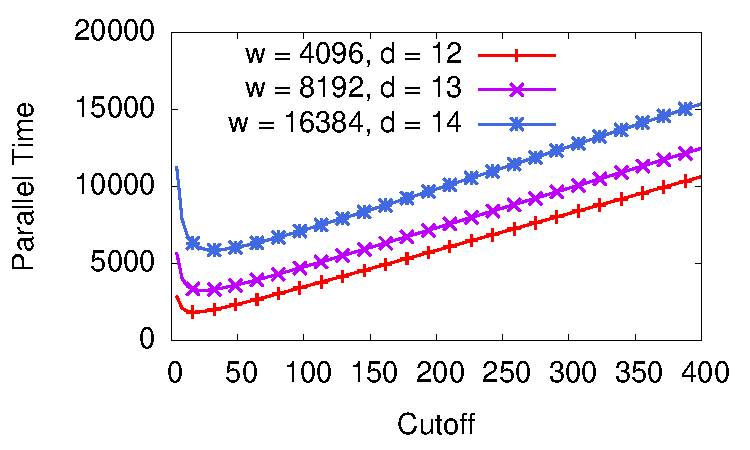
\includegraphics[width=3in]{pictures/plot-run-time-versus-k-multi}

\caption{An illustration of the run-time function $\left(
  1+\frac{\cerr(\csp+\cbal\corc)}{\coff} \right)\,\frac{\sw}{P} \Sc{+}
  (\coff\cerr+\corc+1)\,d$ on $P = 4$ processors with constants $\cerr =1$,
   $\csp = 5$, $\cbal = 1$, and $\corc = 2$, and different work and
  depth values.}

\label{fig:run-time-versus-kappa}
\end{figure}

\thmref{orc-time-bound} shows that the running time of a parallel
program can be controlled by changing the constant $\coff$; the
formula, however, reveals an interesting tradeoff: we can reduce
task-creation overheads but this comes at the cost of increasing the
depth.  To see this connection better, consider the bound
that appears in the statement of \thmref{orc-time-bound}
%$$
%\left( 1+\frac{\cerr(\csp+\creg\corc)}{\coff} \right)\frac{\sw}{P}
%\Sc{+} \left( \coff\cerr + \corc + 1\right)d$$
and notice that as \coff increases the work (first) term decreases
but the depth (second) term increases.  \figref{run-time-versus-kappa}
illustrates a concrete instance of the bound for a hypothetical
computation for fixed constants but different raw work and raw depth.
The exact values of the constant and the raw work and depth are not
relevant to our discussion; constants are fixed at some reasonable
values consistent with our experimental observations.  The work and
depth are consistent with a program whose raw work is linear
in the input size
and whose raw depth is logarithmic in the input size.

As \figref{run-time-versus-kappa} illustrates, the parallel run time
decreases as we increase \coff up to some inflection point and then
starts increasing.  
%ARTHUR: Confirming minimality by checking that the sign of
%the second derivative is positive at the inflection point, 
We compute the optimal value for \coff by solving for the root of the  
derivative. We obtain:
\[
\coff^* = \sqrt{\csp+\creg\corc} \cdot
\sqrt{ \frac{\sw}{P\sd} }.
\]
Thus, with prior knowledge of the raw work and raw depth of a
computation, we can pick \coff to ensure efficiency of parallel
programs.  

Such knowledge, however, is often unavailable.  As we now
show, we can improve efficiency of parallel programs by selecting a
fixed $\coff$ that guarantees that the task creation overheads can be
bounded by any constant fraction of the raw work, without increasing
the depth of the computation significantly. 

%The idea is to make sure that $\coff < \coff^*$, \textit{i.e.}, the cutoff
%remains less than the inflection point.

%\uremark{The constant is not quite universal because it depend on
%  \cbal.  Let's revisit this issue after arthur does a pass on the
%  analysis.}


%\aremark{This theorem and its proof will be polished.}
\begin{theorem}[Run time with fixed $\coff$]
\label{thm:task-creation-overheads}
Consider an oracle with $\corc$ cost and $\cerr$ error.
For any $\cbal\geq 1$ and for any constant $r$ such that $0 < r < 1$,
there exists a constant $\coff$ and a constant $c$
such that the evaluation with 
the oracle semantics of a $\cbal$-balanced program 
reduces task creation overheads to a fraction $r$ of the
raw work, while in the same time increasing the total depth 
by no more than a factor $\frac{c}{r}$.
With a greedy scheduler, the total parallel
run time on $P$ processors of such a program
therefore does not exceed
$(1 + r) \frac{\sw}{P} + \frac{c}{r}\, \sd$.  
%
%When the raw work is a function asymptotically greater than raw depth,
%the increase in depth is not significant: for all but a constant
%number of inputs the total run-time improves over when $\coff = 0$,
%where all parallel tasks are executed in parallel.
\end{theorem}
\begin{proof}
Consider a particular $\cbal$-balanced program 
with raw work $\sw$ and raw depth $\sd$,
%and let $\sw$ denote its raw work and $\sd$ denote its raw depth.
and consider its evaluation under the oracle semantics.  
%
By \thmref{real-orc-work} we know that total work does not exceed
\[
\left(1+\frac{\cerr(\csp+\cbal\corc)}{\coff} \right)\,{\sw}.
\]
To achieve the desired bound on execution time, we take 
 $\coff = \frac{\cerr(\csp + \cbal\corc)}{r}$.
Plugging this value of $\coff$ into the formula
yields~$(1+r)\,{\sw}$ for total work, showing
that task creation overheads are reduced to a fraction $r$ of
the raw work.

Furthermore, by \thmref{real-orc-depth} we know that the total depth 
is bounded by $(\kwmax{\csp}{\cerr\coff}+\corc+1)\,\sd$. Plugging in 
the same value for $\coff$ yields the following bound on total depth:
\[
\sds \Sc\leq \left(\kwmax{\csp}{\frac{\cerr^2(\csp +
    \cbal\corc)}{r}}+\corc + 1\right)\,\sd.
\]
Using $\cerr \ge 1$ and $r < 1$,
we can derive the inequality
\[
\sds \Sc\leq \left(\frac{\cerr^2(\csp + \cbal\corc)}{r}+\frac{\corc+1}{r}\right)\,\sd.
\]
Choosing $c = \cerr^2(\csp + \cbal\corc)+\corc+1$ 
therefore ensures that the total depth does not exceed the desired bound
$\frac{c}{r}\,\sd$.
The run-time bound follows by an application of 
Brent's theorem (\thmref{generalized-brent}). \qed
\end{proof}

This final theorem enables us to reduce task creation overheads to any
desired constant fraction of the raw work by choosing a $\coff$ that
is independent of the specific inputs.  This comes at the cost
of increasing the depth, but only by a constant factor of
$\frac{c}{r}$.  In the common case, when the work is
asymptotically greater than depth, \textit{e.g.}, $\Theta(n)$ versus
$O(\log{n})$, the resulting run-time guarantees that the increase in
depth remain small: specifically, the depth term itself is a fraction
of the work term for all but a constant number of small inputs.  


%% Finally, to show that choosing $r > 0$ improves the run-time for
%% most inputs, we prove that $\coff < \coff^*$ for all but a constant
%% number of inputs when there is an asymptotic gap between work and
%% depth.  The inequality $\coff < \coff^*$ holds if $ \frac{\cerr(\csp +
%%   \cbal\corc)}{r} < \sqrt{\frac{\cerr (\csp+\creg\corc)}{\cerr+1}}
%% \cdot \sqrt{ \frac{\sw}{P\sd}}.  $ Using basic algebra, we deduce that
%% the inequality holds if $r^2 > \cerr(\cerr+1)(\csp + \cbal\corc)
%% \frac{P\sd}{\sw}$.  This can be read simply as $r^2 > c'
%% \frac{P\sd}{\sw}$, where $c'$ is the appropriate constant.  Thus, if
%% there is an asymptotic gap between work and depth, that is
%% $\frac{\sd}{\sw} = o(1)$, then $\frac{\sw}{\sd}$ will increase
%% monotonically with the input size and thus $\coff < \coff^*$ for all
%% input sizes except for some constant number.\qed



\subsection{Balanced programs}
\label{sec:balanced}

Our bounds with the realistic oracle hold only for what we called
$\cbal$-balanced programs, where the oracle is not called on small
tasks.  This assumption can be satisfied by calling the oracle
``regularly.''  It seems likely that this assumption would hold for
many programs without requiring any changes to the program code.  In
this section, we show that recursive, divide-and-conquer programs are
$\cbal$-balanced.

To that end, we introduce the notion of $\cbal$-regularity.
Intuitively, a program is $\cbal$-regular if, between any two calls
to the oracle involved in the execution of this program,
the amount of work does not reduce by more than a factor $\cbal$.
We will then establish that any $\cbal$-regular program is 
a $\cbal$-balanced program.
Before giving the formal definition of $\cbal$-regularity,
we need to formally define what it means for a parallel tuple
to be dominated by another parallel tuple.

\begin{comment}
\uremark{Arthur, I am leaving this to you to complete. Old text follows.}
Fortunately, most programs do not exhibit this pathological behavior.
However, to prove a better bound we need to make further assumptions
about the structure of the program. It turns out that a sufficient
condition for establishing an interesting bound is to ensure
that the oracle is never called on too small tasks.
This property is hard to capture in a hardware-independent way.
However, we can devise a sufficient condition, called {\em regularity},
which is hardware-independent and ensures the desired property. 
Intuitively, a program is $\creg$-regular if the ratio between 
the work involved in a recursive call and the work involved
in the next recursive call does not exceed $\creg$.
Divide-and-conquer algorithm typically satisfy the regularity 
condition. We next formalize the definition of regularity.
\end{comment}

%------------------------
\begin{definition}[Domination of a parallel branch]
A branch $e$ of a parallel tuple is said to be {\em dominated} by the
branch $e_i$ of another parallel tuple $\kwpt{e_1}{e_2}$ if
the expression $e$ is involved in the execution of the branch $e_i$.
\end{definition}
%------------------------

%------------------------
\begin{definition}[Regularity of a parallel program]
A program is said to be $\creg$-regular if,
for any parallel branch involving, say, $\sw$ units of raw work, 
either $\sw$ is very large compared with $\coff/(\cerr\creg)$
or this branch is dominated by another parallel branch
that involves less than $\creg\sw$ units of work.
\end{definition}
%------------------------
%
The condition ``$\sw$ is very large compared with $\coff/(\cerr\creg)$''
is used to handle the outermost parallel tuples, which are not
dominated by any other tuple. 

Note that the regularity of a program is always greater than $2$.
Indeed, if one of the branch of a parallel tuple is more
than half of the size of the entire tuple, then the other 
branch must be smaller than half of that size.
On the one hand, algorithms that divide their work in 
equal parts are $\creg$-regularity with $\creg$ very close to $2$.
On the other hand, ill-balanced programs can have a very
high degree of regularity. Observe that every program is $\infty$-regular.

%------------------------
%\begin{example}[Regularity in a complete binary tree] ~\\
For example, consider a program that traverses a complete binary tree
in linear time. A call on a tree of size $n$ 
has raw work \W{nc}, for some constant $c$.
If the tree is not a leaf, its size $n$ has to be at least $3$.
The next recursive call involves raw work \W{\floorfrac{n-1}{2} c},
The ratio between those two values is equal $n / \floorfrac{n-1}{2}$.
This value is always less than $3$ when $n\geq 3$.
So, the traversal of a complete binary tree is a 3-regular algorithm.
%\end{example}
%------------------------

%------------------------
%\begin{example}[Regularity in mergesort]
%Consider the mergesort algorithm. A recursive call on $2n+1$ values
%has raw work \Q{c n \log n}, for some constant $c$.
%A recursive call is performed if $n$ is equal to three or more.
%immediately nested has 
%at least raw work \Q{c \floorfrac{n-1}{2} \log \floorfrac{n-1}{2}},
%So, the ratio between the work of two successive parallel branches is at most:
%$$\frac{c n \log n}{c \floorfrac{n-1}{2} \log \floorfrac{n-1}{2}}$$
%In the worst case, $n=3$, the ratio $2.38$.
%So, merge-sort is $2.38$-regular or less.
%\end{example}
%------------------------

The following lemma explains how the regularity assumption
can be exploited to ensure that the oracle is never
invoked on tasks of size less than $\coff/(\cerr\creg)$.
This suggests that, for the purpose of amortizing well the 
costs of the oracle, a smaller regularity is better.

%------------------------
\begin{lemma}[From regularity to balanced]
\label{lem:regularity-elim}~\\
If a program is $\cbal$-regular then it is $\cbal$-balanced.
\end{lemma}
\begin{proof}
We have to show that, during the execution of a $\creg$-regular 
program according to oracle semantics, the oracle is
never invoked on subexpressions involving less than $\coff/(\cerr\creg)$
raw work.
Consider a particular subexpression $e$ involving $\sw$ units of raw work,
and assume that the oracle is invoked on this subexpression.
Because the oracle is being invoked, $e$ 
must correspond to the branch of a parallel tuple.
By the regularity assumption, either $\sw$ is very
large compared with $\coff/(\cerr\creg)$, in which case
the conclusion holds immediately, or the branch $e$
is dominated by a branch $e_i$ that involves that 
involves $\sw'$ units of work, with $\sw' \leq \creg\sw$.
For the latter case, we need to establish $\sw \geq \coff/(\cerr\creg)$.
To that end, it suffices to prove that $\sw' \geq \coff/\cerr$,
which amounts to showing that the amount of raw
work associated with the dominating branch $e_i$
contains at least $\coff/\cerr$ raw work. 

We conclude the proof by establishing the inequality $\sw' \geq \coff/\cerr$.
Because the oracle is being invoked on the subexpression $e$,
it means that $e$ is being evaluated in the mode $\sorc$. Therefore,
the call to the oracle on the dominating branch $e_i$ must have 
predicted $e_i$ to contain more than $\coff$ raw work.
(Otherwise $e_i$ and its subexpression $e$ would have both
been executed in the sequential mode.)
Given that the oracle makes error by no more than a factor $\cerr$,
if $e_i$ is predicted to contain more than $\coff$ units of raw work, 
then $e_i$ must contain at least $\coff/\cerr$ units of raw work. 
So, $\sw' \geq \coff/\cerr$. \qed
\end{proof}
%------------------------
